
接下来,将要了解各种性能分析工具。我们已经了解了性能分析器的使用,可以确定占用大量计算时间的函数。这正是其用途所在,它可以用来查找“热点”函数和代码段。

有许多不同的商业和开源分析工具可用。本节中,我们将研究两个在Linux系统上主流的性能分析器。这里不是想要将读者培养成某个特定工具的专家,而仅是了解选择使用的性能分析器可以提供什么,以及如何对其结果进行解析。

首先,了解一下几种不同类型的性能分析器:

\begin{itemize}
\item 一些分析器在解释器或虚拟机下执行,并观察各个代码段所花费的时间。这些分析器的主要缺点是,程序运行的速度比直接编译到机器指令的代码慢。对于像C++这样的编译语言来说,并且通常不会在虚拟机下运行的。

\item 还有一些分析器,要求在编译或链接期间用特殊的指令插入代码中。这些指令为分析器提供了相应的信息,例如:当函数调用或循环开始和结束时,会告知数据收集引擎。这些分析器比前一种类型的分析器快,但仍然比本机执行速度慢。并且,需要对代码进行特殊编译,并依赖于某种假设:插装的代码与原始代码的性能差异不大(相对的)。

\item 大多数现代分析器使用现代CPU上的硬件计数器。这些是硬件寄存器,可以用来跟踪某些硬件事件,硬件事件就是执行指令。可以看到这对分析非常有效:处理器将做计数指令的工作,而不需要其他工具或任何开销。我们要做的就是读取计数寄存器的值。

\end{itemize}

或者,用简单地计算复杂指令的方法。我们需要知道在每个函数中,甚至在每一行代码执行所花费的时间。如果分析器在执行每个函数(或每个循环、每一行代码等)前后读取指令计数,就可以做到这一点。这就是为什么有分析器可以使用多种计数方案:使用特定的指令标记感兴趣的代码段,并使用硬件性能计数器来进行实际测量。

有些分析器依赖于时间采样,其以一定的间隔中断程序,例如:每10毫秒中断一次,并记录性能计数器的值,以及程序的当前位置(即将执行的指令)。如果90\%的样本在调用\texttt{compare()}函数的过程中获得的,则可以假设程序花了90\%的时间进行字符串比较,这种方法的准确性取决于采样数和采样率。

对程序执行的采样越频繁,收集的数据就越多,但开销也会越大。某些情况下,在采样不太频繁的情况下,可以使用硬件分析器,这就对程序的运行时间没有任何影响了。

\subsubsubsection{2.4.1\hspace{0.2cm}perf分析器}

本节中的第一个分析器工具是Linux性能分析器。这是Linux上最流行的分析器之一,大多数发行版都有安装了,其是基于硬件性能计数器和基于时间采样的分析器。

运行这个分析器最简单的方法是收集整个程序的计数器值,可以通过\texttt{perf stat}命令完成:

%\hspace*{\fill} \\ %插入空行
\begin{center}
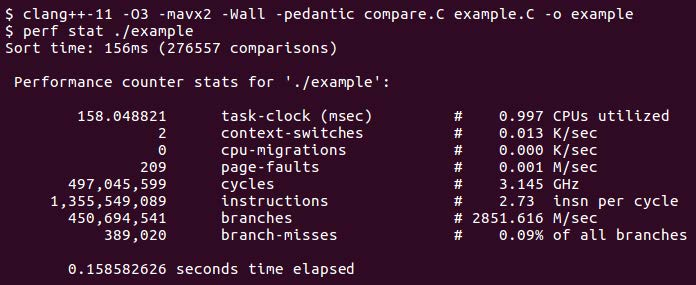
\includegraphics[width=0.9\textwidth]{content/1/chapter2/images/6.jpg}\\
图 2.6
\end{center}

从图2.6中可以看到,编译不需要任何特殊选项或工具。程序由分析器执行,\texttt{stat}选项告诉分析器显示在程序运行期间,硬件性能计数器中累积的计数值。本例中,程序运行了158毫秒(与程序本身打印的时间一致),并执行了13亿多条指令。还显示了其他几个计数器,如“页面错误”和“分支”。这些计数器是什么,还有哪些计数器可用?

事实证明,现代CPU可以收集不同类型事件的统计信息,但一次只能收集几种类型的事件。前面的例子中,展示了8个计数器,因此可以假设这个CPU有8个独立的计数器。以前,每个计数器都会分配到一个事件类型中。分析器本身可以列出所有已知的事件,并可以计数:

%\hspace*{\fill} \\ %插入空行
\begin{center}
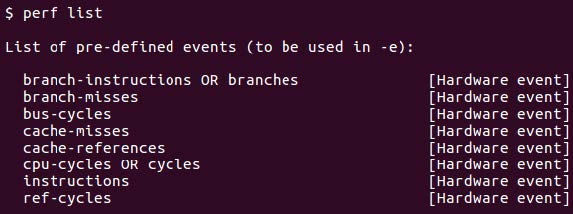
\includegraphics[width=0.9\textwidth]{content/1/chapter2/images/7.jpg}\\
图 2.7
\end{center}

图2.7中的列表是不完整的,可用的计数器因CPU而异(如果使用虚拟机,则在类型和配置上有所不同)。图2.6中的结果只是默认配置的计数器收集的,我们还可以选择其他的计数器进行配置:

%\hspace*{\fill} \\ %插入空行
\begin{center}
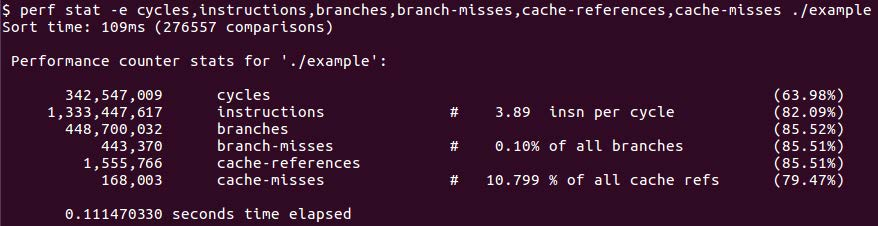
\includegraphics[width=0.9\textwidth]{content/1/chapter2/images/8.jpg}\\
图 2.8
\end{center}

图2.8中,我们可以测量CPU周期和指令,以及分支、分支缺失、缓存引用和缓存缺失。下一章将详细解释这些计数器和其相应的监视事件。

简单地说,周期时间是CPU频率的倒数,所以一个3GHz的CPU每秒可以运行30亿个周期。大多数CPU的频率是可变的,这使得测量变得更复杂了。因此,为了精确的分析和进行基准测试,建议禁用省电模式和其他会让CPU时钟变化的功能。指令计数器测量处理器执行指令的数量,CPU平均每周期可以执行四条指令。

“分支”是条件指令:每个带有条件的\texttt{if}语句和每个\texttt{for}循环都会生成多条这样的指令。分支缺失在下一章进行解释,现在只能说这是一个性能开销大,而且不受欢迎的事件。

“缓存引用”计算CPU需要从内存中读取的次数。大多数时候是一段数据,比如:字符串中的一个字符。根据处理器和内存的状态,这个取回可以非常快,也可以非常慢。慢的话会认为是“缓存丢失”(“慢”是一个相对概念:相对于3GHz的处理器速度,1微秒是一个很长的时间)。内存层次结构将在后面的章节进行解释,而且缓存丢失也是一个性能开销特别大的事件。

理解了CPU和内存的工作方式后,就能够使用这些指标来衡量程序的总体效率,并确定哪些因素限制了程序的性能。

目前为止,我们只看到了整个项目的测量结果。图2.8中表明哪些事件拖累了代码的性能,例如:如果现在接受“缓存丢失”对性能不利的观点,可以推断出这段代码的主要问题是低效的内存访问(十分之一的内存访问是缓慢的)。然而,代码具体是哪部分导致了较差的性能,这种类型的数据并没有展示出来。为此,不仅需要在程序执行前后收集数据,还需要在程序执行期间收集数据。来看看如何用\texttt{perf}来收集这些信息。

\subsubsubsection{2.4.2\hspace{0.2cm}使用perf进行详细分析}

\texttt{perf}分析器将硬件计数器与基于时间采样结合,记录正在运行程序的性能情况。对于每个示例,记录程序计数器的位置(要执行的指令的地址)和需要查看的性能计数器。运行后对数据进行分析,包含大多数的函数和代码行的执行时间。

分析器的数据收集不会特别复杂。在运行时,收集指令地址转换为原始源代码中的行号,程序必须使用调试信息进行编译。若已经习惯了“优化”和“非优化”这两种编译模式,这种编译器选项的组合可能会出乎意料,这时“优化”和“非优化”都会启用。启用后者的原因是,我们需要在生产环境中运行的相同代码;否则,数据没什么无意义。所以需要通过编译代码来分析,并使用\texttt{perf record}命令运行分析器:

%\hspace*{\fill} \\ %插入空行
\begin{center}
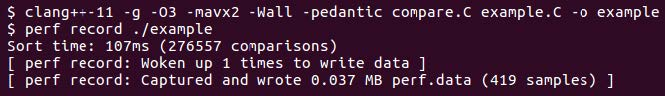
\includegraphics[width=0.9\textwidth]{content/1/chapter2/images/9.jpg}\\
图 2.9
\end{center}

与\texttt{perf stat}类似,可以指定计数器或一组计数器。但这次,使用默认计数器。我们没有具体说明采样的频率,也使用默认值。采样频率可以显式指定,例如:\texttt{perf record -c 1000}即记录每秒1000个样本。

运行程序后,屏幕输出包括常规输出和分析器的信息。上一个例子中,分析样本已经捕获到名为\texttt{perf.data}的文件中(这是也可以修改)。为了将文件中的数据可视化,需要使用数据分析工具,就是\texttt{perf report}。运行此命令后,界面如下所示:

%\hspace*{\fill} \\ %插入空行
\begin{center}
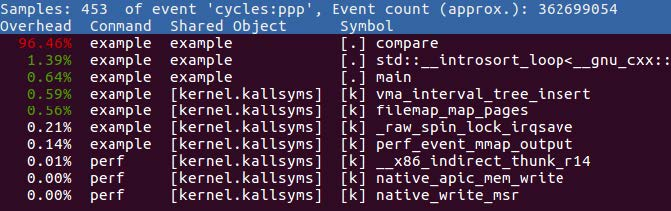
\includegraphics[width=0.9\textwidth]{content/1/chapter2/images/10.jpg}\\
图 2.10
\end{center}

这就是对数据的分析,按函数执行时间占总时长占比进行排序。可以深入到函数内部,了解哪一行代码执行的时间最长:

%\hspace*{\fill} \\ %插入空行
\begin{center}
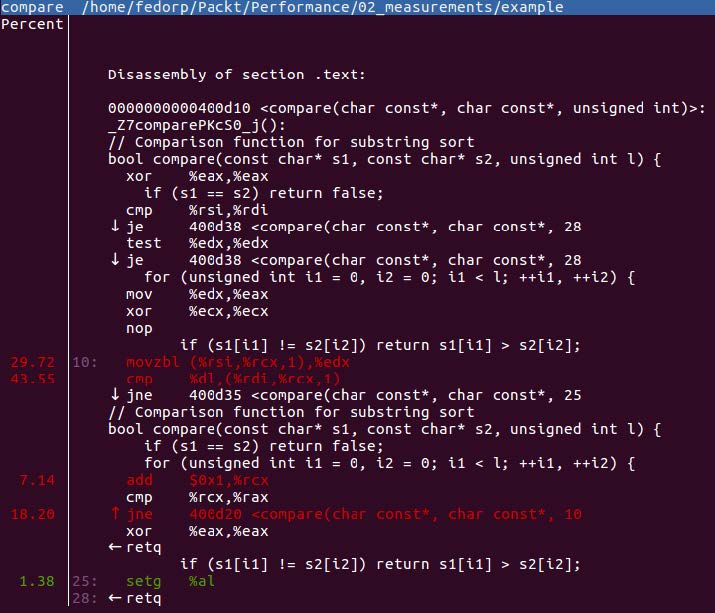
\includegraphics[width=0.9\textwidth]{content/1/chapter2/images/11.jpg}\\
图 2.11
\end{center}

图2.11左边的数字是每一行执行时间的百分比。这条“线”说明了什么?其显示了源代码和产生的汇编指令,执行时间计数器与每个硬件指令相关联(这是CPU执行的指令,所以这是可计数的)。编译后的代码可以和源代码进行关联,这种关联是由分析器使用调试信息建立的。然而,因为对代码进行了优化,所以这种对应并不准确。编译器在编译时对原始代码进行优化,这些优化会导致代码重排,并可能改变计算的方式。即使在这个简单的例子中也可以看到一个很诡异的现象:下面的源码行出现了两次。

\begin{lstlisting}[style=styleCXX]
if (s1 == s2) return false;
\end{lstlisting}

原因是这一行生成的指令并不都在同一个地方;优化器将它们与来自其他行的指令重新排序。因为这两条指令最初由它生成,所以分析器将这行源码显示在两条机器指令附近。

即使不看汇编程序,我们也可以知道,时间花在比较字符和运行循环上,以下两行源码占用了大部分时间:

\begin{lstlisting}[style=styleCXX]
for (unsigned int i1 = 0, i2 = 0; i1 < l; ++i1, ++i2) {
	if (s1[i1] != s2[i2]) return s1[i1] > s2[i2];
\end{lstlisting}

为了充分利用这些数据,至少有助于理解当前使用平台(在我们的例子中是x86 CPU)的汇编语言。分析器还提供了一些有助于分析的工具,例如:通过将光标放在\texttt{jne}(如果不是等于的话跳转)指令上,可以跳转到哪里,以及与跳转相关的条件:

%\hspace*{\fill} \\ %插入空行
\begin{center}
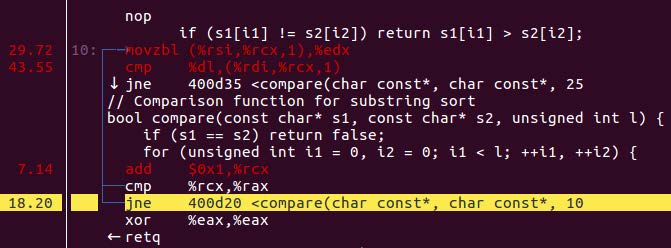
\includegraphics[width=0.9\textwidth]{content/1/chapter2/images/12.jpg}\\
图 2.12
\end{center}

这看起来会重复跳转最后几行代码,所以跳转前面的\texttt{cmp}(compare)指令必须是\texttt{i1 < l},跳转和比较总共占了执行时间的18\%,所以之前对(不必要的)比较操作的关注是合理的。

\texttt{perf}分析器有很多的选项和功能来分析、过滤和合并结果,可以从其文档中了解更具体的内容(这个分析器也有几个GUI前端)。接下来,我们将快速了解另一个分析器,来自谷歌的性能工具。

\subsubsubsection{2.4.3\hspace{0.2cm}谷歌的性能分析器}

谷歌CPU分析器使用硬件性能计数器,也需要代码的链接时按插指令(但编译时不需要)。要准备代码进行分析,必须将与分析器的库进行链接:

%\hspace*{\fill} \\ %插入空行
\begin{center}

\includegraphics[width=0.9\textwidth]{content/1/chapter2/images/13.jpg}\\
图 2.13
\end{center}

图2.13中,这个库是由\texttt{-lprofiler}指定的。与perf不同,这个分析器不需要任何特殊工具来调用程序,因为相应的代码已经链接到可执行文件中。可检测的可执行文件不会自动开始分析,必须通过设置环境变量\textit{CPUPROFILE}为要存储结果的文件指定路径。其他选项也通过环境变量来控制(不用命令行选项),例如:通过变量\texttt{CPUPROFILE\_FREQUENCY}设置每秒采样数:

%\hspace*{\fill} \\ %插入空行
\begin{center}
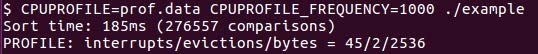
\includegraphics[width=0.9\textwidth]{content/1/chapter2/images/14.jpg}\\
图 2.14
\end{center}

同样,我们看到了程序本身和分析器的输出,并得到了必要的数据文件。该分析器有交互式和批处理两种模式,其交互模式是一个简单的文本界面:

%\hspace*{\fill} \\ %插入空行
\begin{center}
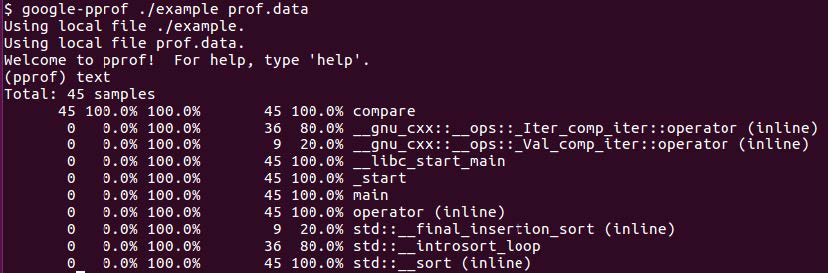
\includegraphics[width=0.9\textwidth]{content/1/chapter2/images/15.jpg}\\
图 2.15
\end{center}

只需以可执行文件和数据文件的名称作为参数运行\texttt{google-pprof}(通常只安装为\texttt{pprof}),就会弹出命令提示符。这里,可以得到用执行时间百分比标注的函数信息,可以在源代码级别进一步分析程序性能:

%\hspace*{\fill} \\ %插入空行
\begin{center}
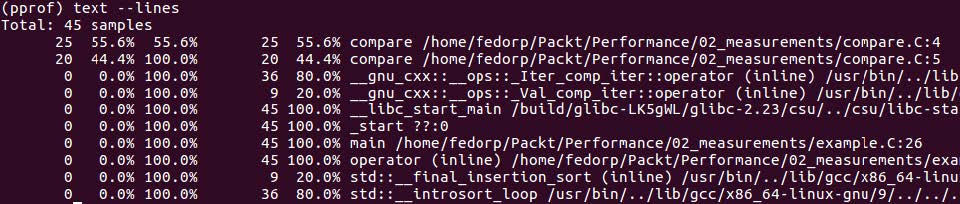
\includegraphics[width=0.9\textwidth]{content/1/chapter2/images/16.jpg}\\
图 2.16
\end{center}

这个分析器采用了不同的方法,并且不会立即深入到机器代码中(尽管也可以生成带注释的汇编码)。尽管表面上的看起来简单,其实不然。前面提到的优化警告仍然存在,编译器仍然会对代码进行优化(指令重排)。

由于作者实现的方法不同,不同的分析器就有不同的优缺点。为了不将这一章变成分析器手册,我们将在本节的其余部分展示在收集和分析数据文件时,可能遇到的问题。

\subsubsubsection{2.4.4\hspace{0.2cm}使用调用图进行分析}

目前为止,简单示例规避了实际中在每个程序中都会遇到的问题。我们看到比较函数占了大部分的执行时间,这样就能立即知道程序的哪个部分非常耗时,因为这个函数只有这一行代码。

现实中的程序都没有这么简单,编写函数的主要原因是便于重用。显然,许多函数在多个位置上都有调用,有些是多次,有些可能只有几次,不同的调用通常会使用不同的参数。这样的话,只知道哪个函数花费大量时间就不够了,还需要知道使用这个函数的上下文(毕竟,最有效的优化可能是少调用性能开销大的函数)。

需要的是一个数据文件,需要报告在每个函数和每行代码中花费了多少时间,而且还显式每个调用链中花费了多少时间。分析器通常使用调用图来显示这些信息。在图中,调用者和被调用者是节点,而调用是边。

首先,我们修改示例,在多个位置调用某个函数。让我们从两种类型的\texttt{sort}调用开始:

\hspace*{\fill} \\ %插入空行
\noindent
\textbf{05\_compare\_timer.C}
\begin{lstlisting}[style=styleCXX]
std::sort(vs.begin(), vs.end(),
  [&](const char* a, const char* b) {
	++count; return compare1(a, b, L); });
std::sort(vs.begin(), vs.end(),
  [&](const char* a, const char* b) {
	++count; return compare2(a, b, L); });
\end{lstlisting}

调用仅在比较函数中不同。我们的例子中,第一个比较函数与前面相同,第二个比较函数的顺序相反。两个函数对子字符串的循环与原来的比较函数相同:

\hspace*{\fill} \\ %插入空行
\noindent
\textbf{05\_compare\_timer.C}
\begin{lstlisting}[style=styleCXX]
bool compare1(const char* s1, const char* s2, unsigned int l) {
	if (s1 == s2) return false;
	for (unsigned int i1 = 0, i2 = 0; i1 < l; ++i1, ++i2) {
		int res = compare(s1[i1], s2[i2]);
		if (res != 0) return res > 0;
	}
	return false;
}
bool compare2(const char* s1, const char* s2, unsigned int l) {
	if (s1 == s2) return false;
	for (unsigned int i1 = 0, i2 = 0; i1 < l; ++i1, ++i2) {
		int res = compare(s1[i1], s2[i2]);
		if (res != 0) return res < 0;
	}
	return false;
}
\end{lstlisting}

两个函数都使用相同的公共函数来比较每个字符:

\begin{lstlisting}[style=styleCXX]
int compare(char c1, char c2) {
	if (c1 > c2) return 1;
	if (c1 < c2) return -1;
	return 0;
}
\end{lstlisting}

实际程序中不会这样做,如果希望避免由于重复循环而造成的代码重复,那么应该编写一个参数化比较字符的函数。无论如何,我们都不想离起始示例太远,希望代码保持简单,以便分析结果。

我们已经准备好生成一个调用图,将显示如何在两个排序调用之间分割字符比较的开销。使用过的两种分析器都可以生成调用图;在本节中,将使用谷歌分析器。分析器收集的数据已经包含了调用链信息,只是还没把它可视化。

我们编译代码,并运行分析器(简单起见,我们把每个函数分别放在不同的源文件中):

%\hspace*{\fill} \\ %插入空行
\begin{center}
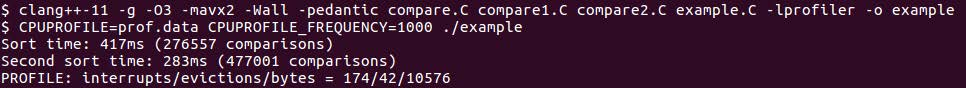
\includegraphics[width=0.9\textwidth]{content/1/chapter2/images/17.jpg}\\
图 2.17
\end{center}

分析器可以以几种不同的格式(Postscript、GIF、PDF等)显示调用图,例如:要生成PDF输出,需要运行以下命令:

\begin{tcblisting}{commandshell={}}
google-pprof --pdf ./example prof.data > prof.pdf
\end{tcblisting}

我们感兴趣的信息在调用图的底部:

%\hspace*{\fill} \\ %插入空行
\begin{center}
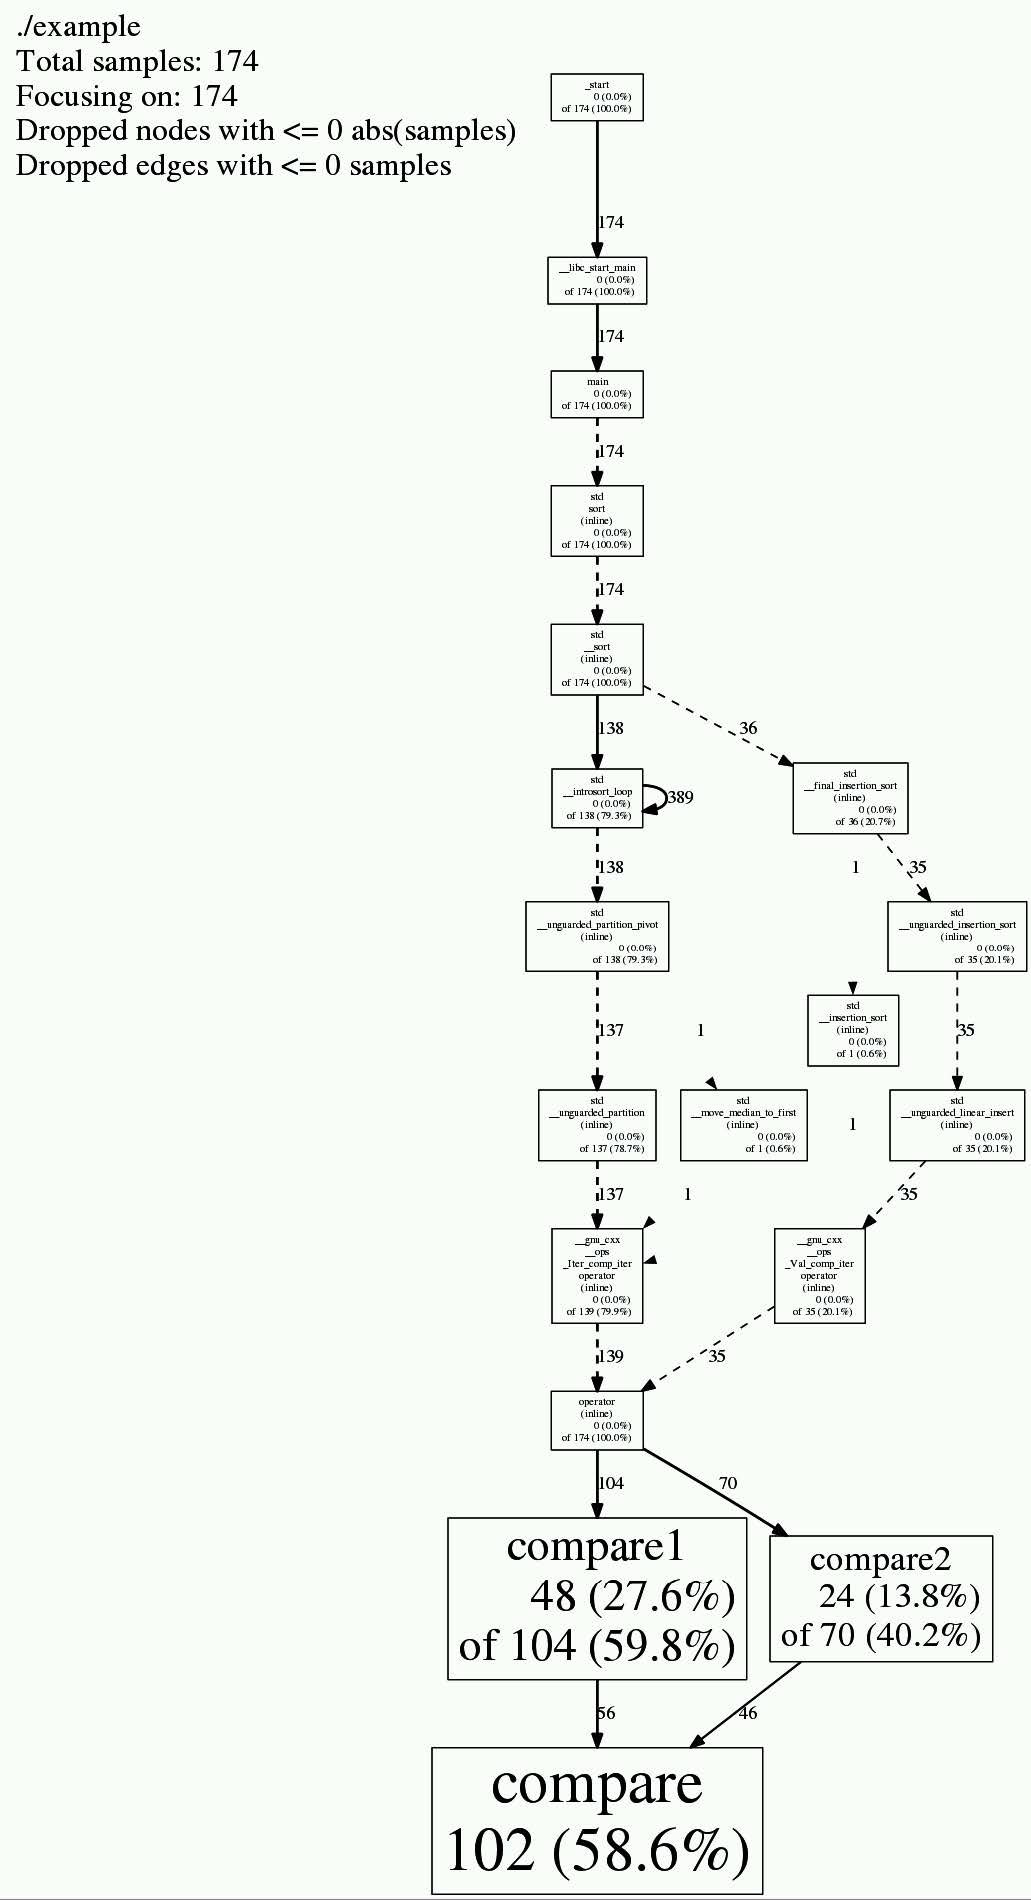
\includegraphics[width=0.6\textwidth]{content/1/chapter2/images/18.jpg}\\
图 2.18
\end{center}

如图2.18所示,\texttt{compare()}函数有两个调用函数,占总执行时间的58.6\%。这两个调用函数中,\texttt{compare1()}函数比\texttt{compare2()}函数调用的次数稍多一些;前者占执行时间的27.6\%(或59.8\%的\texttt{compare()}耗时),后者占13.8\%的时间(或40.2\%的\texttt{compare()}耗时)。

基本调用图通常足以确定问题的调用链,并选择程序需要进一步探索的区域。分析工具还具有更高级的功能,例如:过滤函数名、合并结果等。掌握所选工具的特性可以区分实际和假设。解析性能数据文件可能会比较复杂,原因有很多:一些是由于工具的限制,另一些是更偏向于原理性的解释。下一节中,我们将讨论后一个原因:为了使指标具有相关性,测试必须在完全优化的代码上进行。

\subsubsubsection{2.4.5\hspace{0.2cm}优化和内联}

解析性能数据文件时,我们已经看到了编译器优化是如何搅浑这趟水的:所有的数据文件都是同时生成,并在已编译的机器码上完成的,而我们看到的是程序的源代码。由于编译器优化,这两种形式之间的关系会变得模糊不清。就重新排列源代码而言,最积极的优化方式是函数的编译时内联。

内联要求函数的源代码在调用点是可见的。为了演示,必须将整个源码合并到一个文件中:

\hspace*{\fill} \\ %插入空行
\noindent
\textbf{02\_substring\_sort.C}
\begin{lstlisting}[style=styleCXX]
bool compare(const char* s1, const char* s2, unsigned int l) {
	if (s1 == s2) return false;
	for (unsigned int i1 = 0, i2 = 0; i1 < l; ++i1, ++i2) {
		if (s1[i1] != s2[i2]) return s1[i1] > s2[i2];
	}
	return false;
}
int main() {
	…
	size_t count = 0;
	std::sort(vs.begin(), vs.end(),
	  [&](const char* a, const char* b) {
		++count; return compare(a, b, L); });
}
\end{lstlisting}

现在编译器可以(很可能会)在排序使用比较的地方生成机器代码,而不是调用外部函数。这样的内联是有效的优化方式,当然这种情况经常发生,并不仅仅发生在同一个文件的函数上。更常见的情况是,内联会影响只包含头文件的函数(其整个实现都在头文件中),例如:前面的代码中,对\texttt{std::sort}的调用(看起来像函数调用)肯定是内联的,因为\texttt{std::sort}是模板函数,其整个实现都在头文件中。

我们之前使用的分析器工具是如何处理内联代码的,为带注释的源代码运行谷歌分析器会产生以下报告:

%\hspace*{\fill} \\ %插入空行
\begin{center}
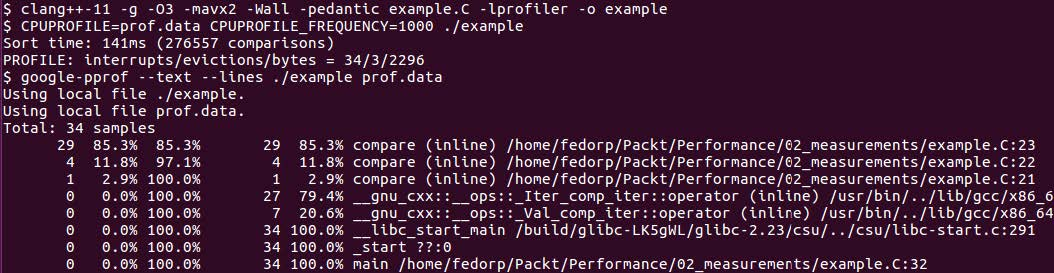
\includegraphics[width=0.9\textwidth]{content/1/chapter2/images/19.jpg}\\
图 2.19
\end{center}

看来分析器知道\texttt{compare()}是内联的,但仍然会显示其原始名称。源代码中的行对应的是函数代码写入的位置,而不是函数调用的位置,例如:第23行是这样的:

\begin{lstlisting}[style=styleCXX]
if (s1[i1] != s2[i2]) return s1[i1] > s2[i2];
\end{lstlisting}

另一方面,perf分析器很难显示内联函数:

%\hspace*{\fill} \\ %插入空行
\begin{center}
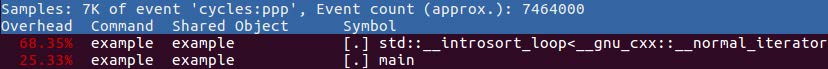
\includegraphics[width=0.9\textwidth]{content/1/chapter2/images/20.jpg}\\
图 2.20
\end{center}

这里,我们可以看到时间似乎花在排序代码和主程序本身上。然而,检查带注释的汇编码可以看到,由\texttt{compare()}函数源码生成的代码,仍占了大多数的执行时间:

%\hspace*{\fill} \\ %插入空行
\begin{center}
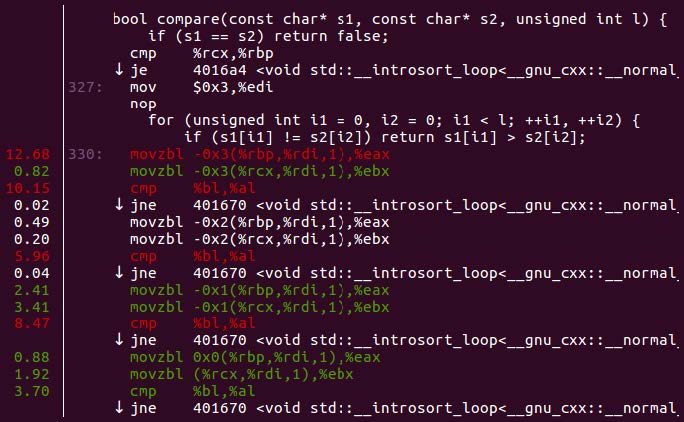
\includegraphics[width=0.9\textwidth]{content/1/chapter2/images/21.jpg}\\
图 2.21
\end{center}

不幸的是,没有简单的方法可以撤消优化对性能数据文件的影响。分析内联、代码重新排序和其他转换的性能,将会转化为一种随实践而发展的技能。现在,给出一些对分析的建议。

\subsubsubsection{2.4.6\hspace{0.2cm}分析建议}

人们可能很容易认为,分析是满足所有性能测试需求的最终解决方案:在分析器下运行整个程序,收集所有数据,并对代码中发生的一切进行分析。不幸的是,这种方法很少奏效。有时,工具的限制会成为障碍。通常,处理大量信息的复杂性太大了。那么,应该如何有效地进行分析呢?

建议是首先收集高级信息,然后进行细化。解析大型模块之间执行时间的数据,可能是一个很好的起点。另一方面,如果这些模块用于基准测试,并且有计时器对所有主要执行步骤进行记录,那么就可以收到到这些信息了。若没有这样的工具,初始的数据文件为这些步骤提供了很好的建议,所以可以现在考虑添加基准测试的工具,以便下次使用,没人会认为一次性就能解决所有的问题吧?

有了基准测试结果和数据的概要,可能会遇到以下几个情况。这个数据文件会指向一些简单的结果,比如:一个花99\%时间做列表的函数。当第一次编写代码时,没有人期望数组的长度超过10个元素,所以只持续了一段时间,然后所有人都忘记了这段代码,直到它出现在数据文件上。

更有可能的是,数据概要文件将引导找到一些大型函数或模块。必须迭代、创建专注于程序有趣部分的测试,并更详细地分析更小的代码部分。一些基准测试数据也有助于解释数据文件:虽然数据文件会说明在给定函数或循环中花费了多少时间,但它不会计算循环迭代或跟踪if-else。大多数分析器都能计数函数调用,所以一个好的模块化代码比一个庞大的代码堆更容易分析。

如果需要收集和细化数据文件,数据会将分析者的注意力集中到代码性能的关键部分。这也是可能会陷入错误的地方:当专注于过慢的代码时,可能会直接优化它,而不考虑其他的情况,例如:数据文件显示某个特定循环在内存分配上花费的时间最多。当决定需要更高效的内存分配时,请考虑是否需要在循环的每个迭代中分配和回收内存。使慢代码变快的最好方法通常是减少调用频率。这可能需要一个不同的算法,或者一个更有效的实现。

通常情况下必须进行计算,这是代码中性能至关重要的部分,加快程序速度的唯一方法是使代码更快。所以必须尝试不同的方法来进行优化,看看哪种方法最有效。可以直接在程序中实现,但这通常是一种浪费时间的方法,会显著降低工作效率。理想情况下,可以快速试验针对特定问题的解决方案,从而提出不同实现或不同算法。这里,可以利用第三种方法来收集性能数据,即微基准测试。













